\documentclass[10pt]{article}
\usepackage[utf8]{inputenc}
\usepackage{mathtools}
\usepackage{graphicx}
\usepackage{array}
\usepackage[margin=0.5in]{geometry}
\usepackage{listings}
\usepackage{color}

\definecolor{mygreen}{rgb}{0,0.6,0}
\definecolor{mygray}{rgb}{0.5,0.5,0.5}
\definecolor{mymauve}{rgb}{0.58,0,0.82}

\lstset{ %
  backgroundcolor=\color{white},   % choose the background color; you must add \usepackage{color} or \usepackage{xcolor}; should come as last argument
  basicstyle=\footnotesize,        % the size of the fonts that are used for the code
  breakatwhitespace=false,         % sets if automatic breaks should only happen at whitespace
  breaklines=true,                 % sets automatic line breaking
  captionpos=b,                    % sets the caption-position to bottom
  commentstyle=\color{mygreen},    % comment style
  deletekeywords={...},            % if you want to delete keywords from the given language
  escapeinside={\%*}{*)},          % if you want to add LaTeX within your code
  extendedchars=true,              % lets you use non-ASCII characters; for 8-bits encodings only, does not work with UTF-8
  frame=single,	                   % adds a frame around the code
  keepspaces=true,                 % keeps spaces in text, useful for keeping indentation of code (possibly needs columns=flexible)
  keywordstyle=\color{blue},       % keyword style
  language=Octave,                 % the language of the code
  morekeywords={*,...},            % if you want to add more keywords to the set
  numbers=left,                    % where to put the line-numbers; possible values are (none, left, right)
  numbersep=5pt,                   % how far the line-numbers are from the code
  numberstyle=\tiny\color{mygray}, % the style that is used for the line-numbers
  rulecolor=\color{black},         % if not set, the frame-color may be changed on line-breaks within not-black text (e.g. comments (green here))
  showspaces=false,                % show spaces everywhere adding particular underscores; it overrides 'showstringspaces'
  showstringspaces=false,          % underline spaces within strings only
  showtabs=false,                  % show tabs within strings adding particular underscores
  stepnumber=2,                    % the step between two line-numbers. If it's 1, each line will be numbered
  stringstyle=\color{mymauve},     % string literal style
  tabsize=2,	                   % sets default tabsize to 2 spaces
  title=\lstname                   % show the filename of files included with \lstinputlisting; also try caption instead of title
}
\renewcommand{\arraystretch}{1.5}
\setcounter{secnumdepth}{0}
\author{Kevin Mambu}
\date{\today}

\title{M1 SESI 2017-2018\\Architecture Multi-Processeurs\\TP4 : Caractérisation
et Dimensionnement des Caches}

\begin{document}
\maketitle

\section{Question C1}
Avec cette configuration, l'execution de la simulation dure 75725 cycles.

\section{Question C2}
Le graphe ci-dessous est l'évolution des taux de MISS sur les caches en fonction
du temps sur une durée de 1000 cycles :
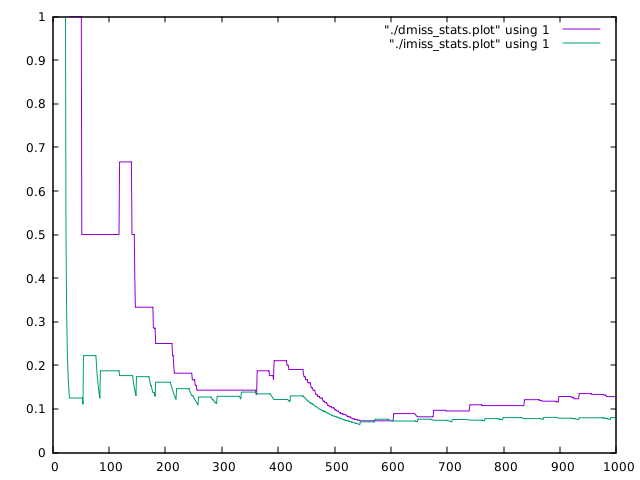
\includegraphics[width=18cm]{overlay_miss_stats.png}\\

\newpage

\begin{itemize}
  \item cycle 20 : Chargement du code du reset depuis la ROM\\
  IMISS RATE = 1.
  \item cycle 30 : Chargement de la première ligne de cache du tableau HexaTab.
  \item cycle 51 : Fin lecture dans le code du reset
  DMISS RATE = 0.5.
  \item cycle 76 : Fin chargement de la première ligne de cache du code du
  main\\IMISS RATE = 0.22
  \item cycle 117 : Fin chargement ligne de cache du main après branchement\\
  IMISS RATE = 0.1875
  \item cycle 140 : Fin lecture de la pile mémoire\\
  Chaque paire de crête IMISS RATE / DMISS RATE peut être apparenté au
  chargement des arguments de sum depuis la pile mémoire
  \item cycle 363 : Lecture deuxième ligne de cache du tableau HexaTab.
  \item cycle 393 : lecture de données non-cachable (tty\_printf)
\end{itemize}

\section{Question C3}
Il y a un signal interne {\it run\_cycles}, correspondant aux nombres de cycles
d'exécutions actives du processeur. Il est égal à
$\frac{c\_total\_cycles}{c\_frz\_cycles}$.\\
Le CPI est égal à $\frac{c\_total\_cycles}{run\_cycles}$.\\
Le taux de MISS d'instructions IMISS RATE est égal à
$\frac{c\_imiss\_count}{run\_cycles}$.\\
Le taux de MISS de données DMISS RATE est égal à
$\frac{{c\_dread\_count}-{c\_dunc\_count}}{run\_cycles}$.\\
c\_dread\_count comptabilise toutes les lectures.

\section{Question D1}

\end{document}
